\documentclass[10pt]{article}
\usepackage[english]{babel}
\usepackage{amsmath}
\usepackage{graphicx}
\usepackage[colorinlistoftodos]{todonotes}
\pagestyle{headings}
\usepackage{indentfirst}
\usepackage[utf8]{inputenc}
\usepackage{xeCJK}
\usepackage{float}

%% Code blocl setting
\usepackage{listings}
\renewcommand{\lstlistingname}{Code}% Listing -> Algorithm
\usepackage{color}

\definecolor{dkgreen}{rgb}{0,0.6,0}
\definecolor{gray}{rgb}{0.5,0.5,0.5}
\definecolor{mauve}{rgb}{0.58,0,0.82}

\lstset{frame=tb,
  language=Python,
  aboveskip=3mm,
  belowskip=3mm,
  showstringspaces=false,
  columns=flexible,
  basicstyle={\small\ttfamily},
  numbers=none,
  numberstyle=\tiny\color{gray},
  keywordstyle=\color{blue},
  commentstyle=\color{dkgreen},
  stringstyle=\color{mauve},
  breaklines=true,
  breakatwhitespace=true,
  tabsize=3
}

\begin{document}

\begin{titlepage}

\newcommand{\HRule}{\rule{\linewidth}{0.5mm}} % Defines a new command for the horizontal lines, change thickness here

\center % Center everything on the page

%----------------------------------------------------------------------------------------
%	HEADING SECTIONS
%----------------------------------------------------------------------------------------

\textsc{\LARGE Shanghai Jiaotong University}\\[1.5cm] % Name of your university/college
\textsc{\Large Big Data Processing Technology}\\[0.5cm] % Major heading such as course name
%\textsc{\large Minor Heading}\\[0.5cm] % Minor heading such as course title

%----------------------------------------------------------------------------------------
%	TITLE SECTION
%----------------------------------------------------------------------------------------

\HRule \\[0.4cm]
{ \huge \bfseries Project 3: Mini DFS}\\[0.4cm] % Title of your document
\HRule \\[1.5cm]

%----------------------------------------------------------------------------------------
%	AUTHOR SECTION
%----------------------------------------------------------------------------------------

\begin{minipage}{0.4\textwidth}
\begin{flushleft} \large
\emph{Author:}\\
% Your name
FEI Yixiao \\118260910031\\
LI Yanhao \\118260910036\\
LUO Dihao \\118260910039\\ % Your name
SHEN Shengyang \\118260910042\\
YAN Shuhan \\118260910050\\ % Your name
\end{flushleft}
\end{minipage}
~
\begin{minipage}{0.4\textwidth}
\begin{flushright} \large
\emph{Supervisor:} \\
Chentao  \textsc{WU} \\% Supervisor's Name
Xin  \textsc{XIE}
\end{flushright}
\end{minipage}\\[2cm]

% If you don't want a supervisor, uncomment the two lines below and remove the section above
%\Large \emph{Author:}\\
%John \textsc{Smith}\\[3cm] % Your name

%----------------------------------------------------------------------------------------
%	DATE SECTION
%----------------------------------------------------------------------------------------

{\large \today}\\[2cm] % Date, change the \today to a set date if you want to be precise

%----------------------------------------------------------------------------------------
%	LOGO SECTION
%----------------------------------------------------------------------------------------


\includegraphics[width=0.5\textwidth]{logo_SPEIT.jpg}\\[1cm] % Include a department/university logo - this will require the graphicx package

%----------------------------------------------------------------------------------------

\vfill % Fill the rest of the page with whitespace

\end{titlepage}
\indent

\section{Introduction}

Our mini-DFS (Distributed File System) is based on Java and is composed with following files:

\begin{itemize}
  \item Main
  \begin{itemize}
    \item Main.java : the client interface
    \item Manager.java : we use this class to store and share basic information among nodes
  \end{itemize}
  \item Node
  \begin{itemize}
    \item DataNode.java : datanode class to perform save/read/recover functions
    \item NameNode.java : namenode class to perform load/ls/split/read/fetch functions
  \end{itemize}
  \item Tools
  \begin{itemize}
    \item Block.java : class to store file block's information
    \item FileHelper.java : class to read/write/recover file blocks
    \item FileMap.java : class to store file mapping information
    \item MyFile.java : class to store file information (containing several blocks)
    \item Operation.java : class storing different operations including ls,put,fetch,read,quit,recover
  \end{itemize}
\end{itemize}

\subsection{Usage}

Users can access Mini-DFS by directly running Main.java.

\begin{itemize}
  \item ls : show list of files
  \item put source\_file\_path : upload local file to mini-DFS
  \item read file\_ID : read the first block of required file
  \item fetch file\_id save\_path : download file from mini-DFS to local file system
  \item recover file\_id : try to recover file block if some datanode lost file blocks
  \item quit : exit Mini-DFS
\end{itemize}


\section{Architecture}

\begin{figure}[H]
\centerline{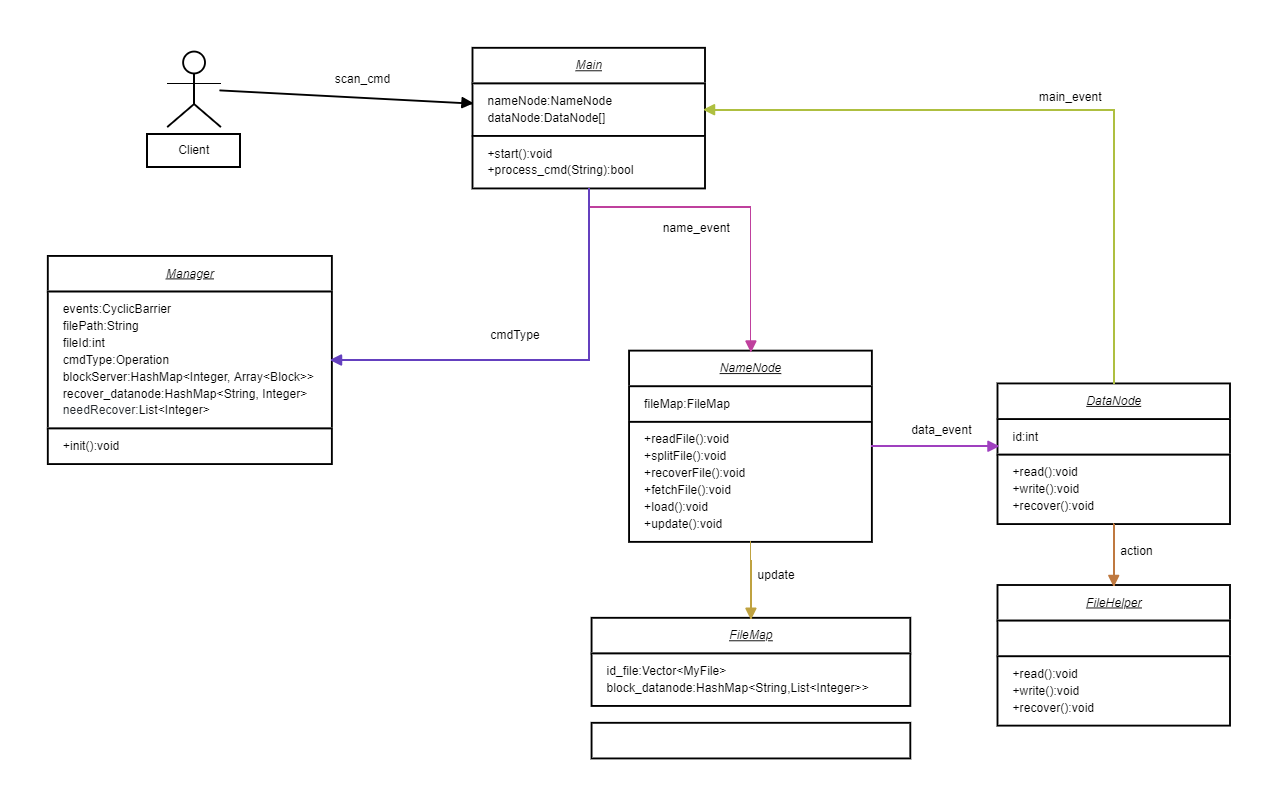
\includegraphics[width = 1.5\textwidth]{screenshot//process.png}}
\caption{Architecture}
\label{fig_process}
\end{figure}

As we can see from the image, when a client type some command to the interface \textit{Main},
\textit{Main} share this command with \textit{NameNode} and \textit{DataNode} through \textit{Manager}.
 At the same time, we use \textit{java.util.concurrent.CyclicBarrier} \textit{name\_event},
 \textit{main\_event}, \textit{data\_event} to send signal from \textit{Main} to \textit{NameNode} and
 \textit{DataNode}. So, then \textit{Main} uses name\_event.await() to notify \textit{NameNode} to do command,
 \textit{NameNode} uses data\_event.await() to notify \textit{DataNode} to do command, finally \textit{DataNode}
 uses main\_event.await() to notify \textit{Main} that all process has been done and it can receive next command from client.

\section{Example}

As you may discover during the experiment, our Mini-DFS accepts only several commands. When the command line does not understand
the command, it gives the list of the accepted commands. In addition, each command has its own format of the input. The input number of
arguments might be different, so when the format is not correct, it also gives the warning message to help the client enter the correct commands.\\
Now first, we upload a file to Mini-DFS using \textit{put}.

\begin{figure}[H]
\centerline{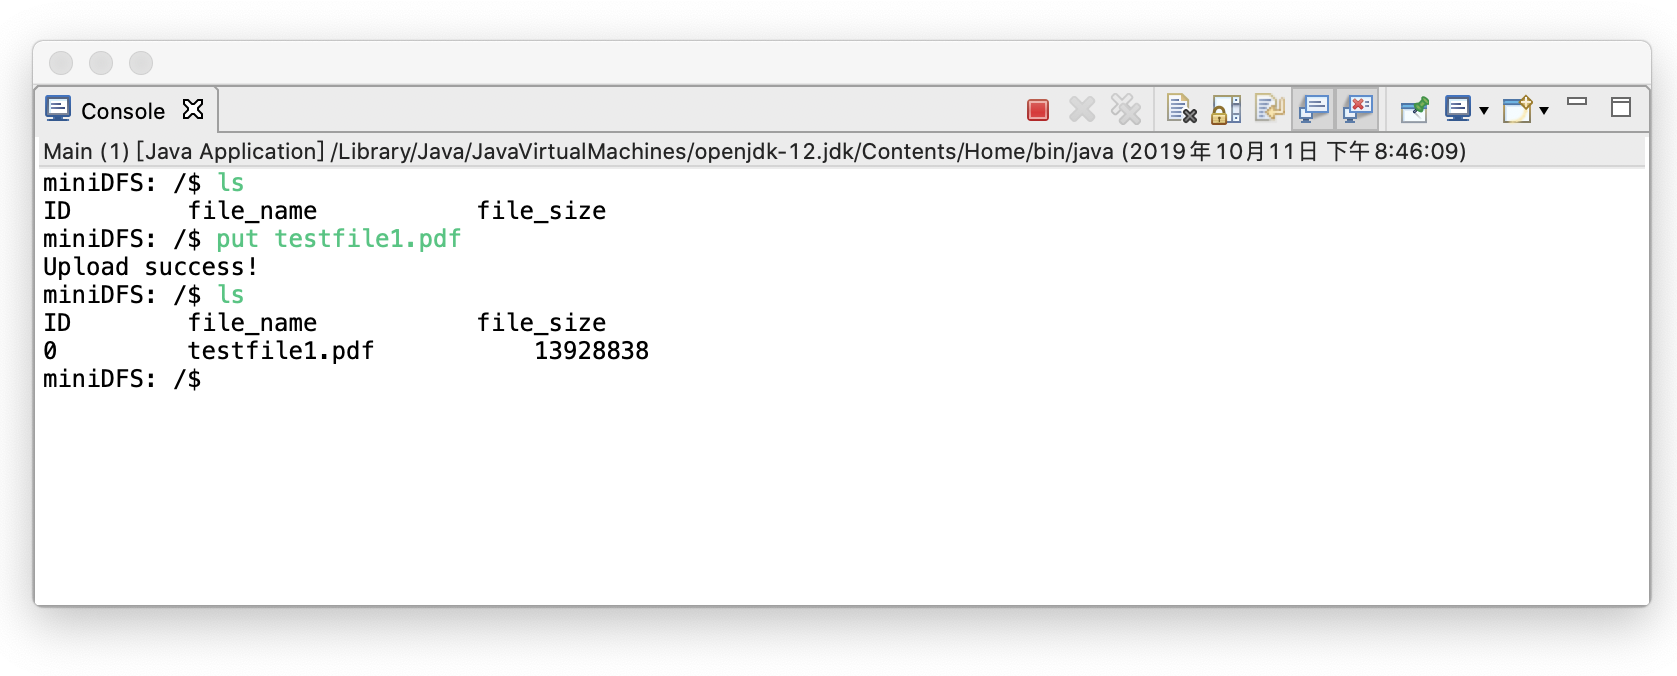
\includegraphics[width = 1\textwidth]{screenshot//put_01.png}}
\caption{Usage: put}
% \label{fig_process}
\end{figure}

In directory \textit{dfs}, we can see that it creates seven blocks and duplicates them for 3 times distributed uniformly among four datanodes.

\begin{figure}[H]
\centerline{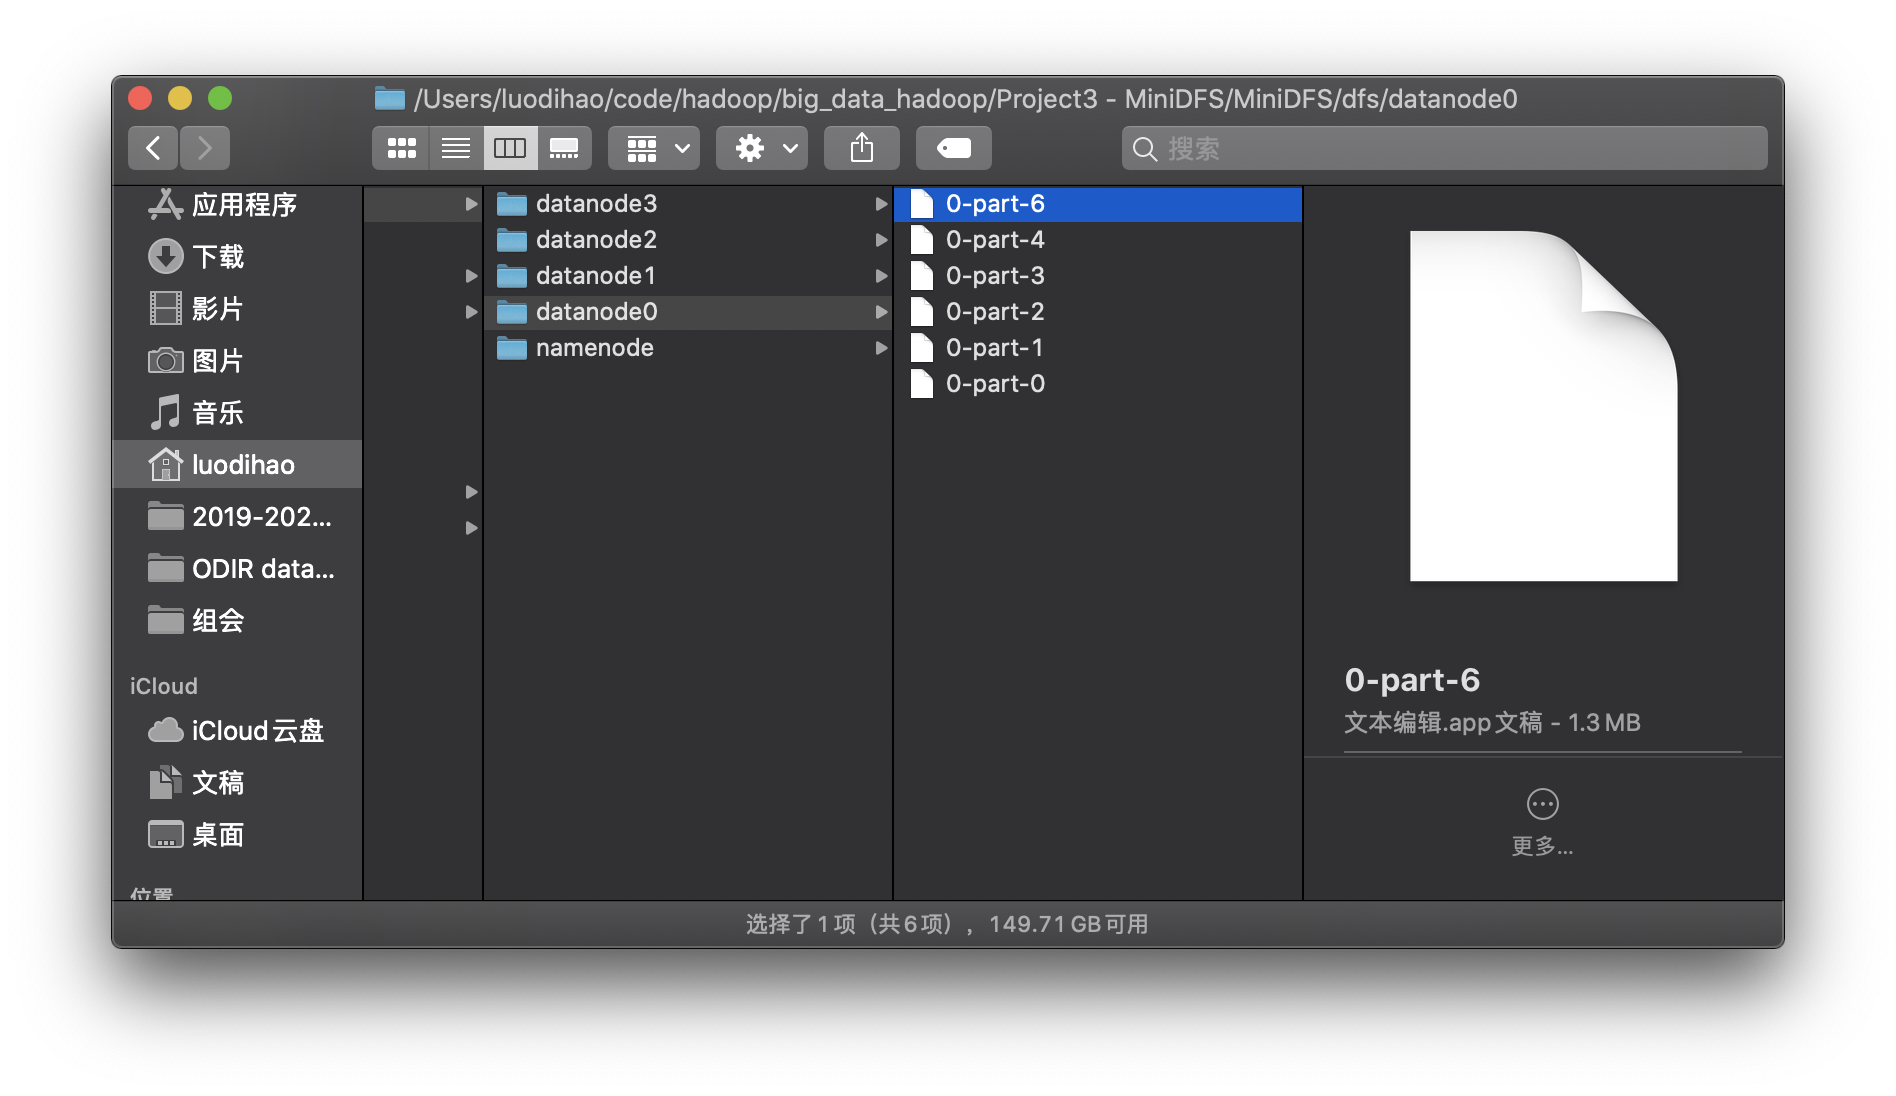
\includegraphics[width = 1\textwidth]{screenshot//put_02.png}}
\caption{Usage: put}
% \label{fig_process}
\end{figure}

Then, we can try to read the first block of this file. Since it's of format pdf, it seems to be unreadable strings, but it works if this is a text file.

\begin{figure}[H]
\centerline{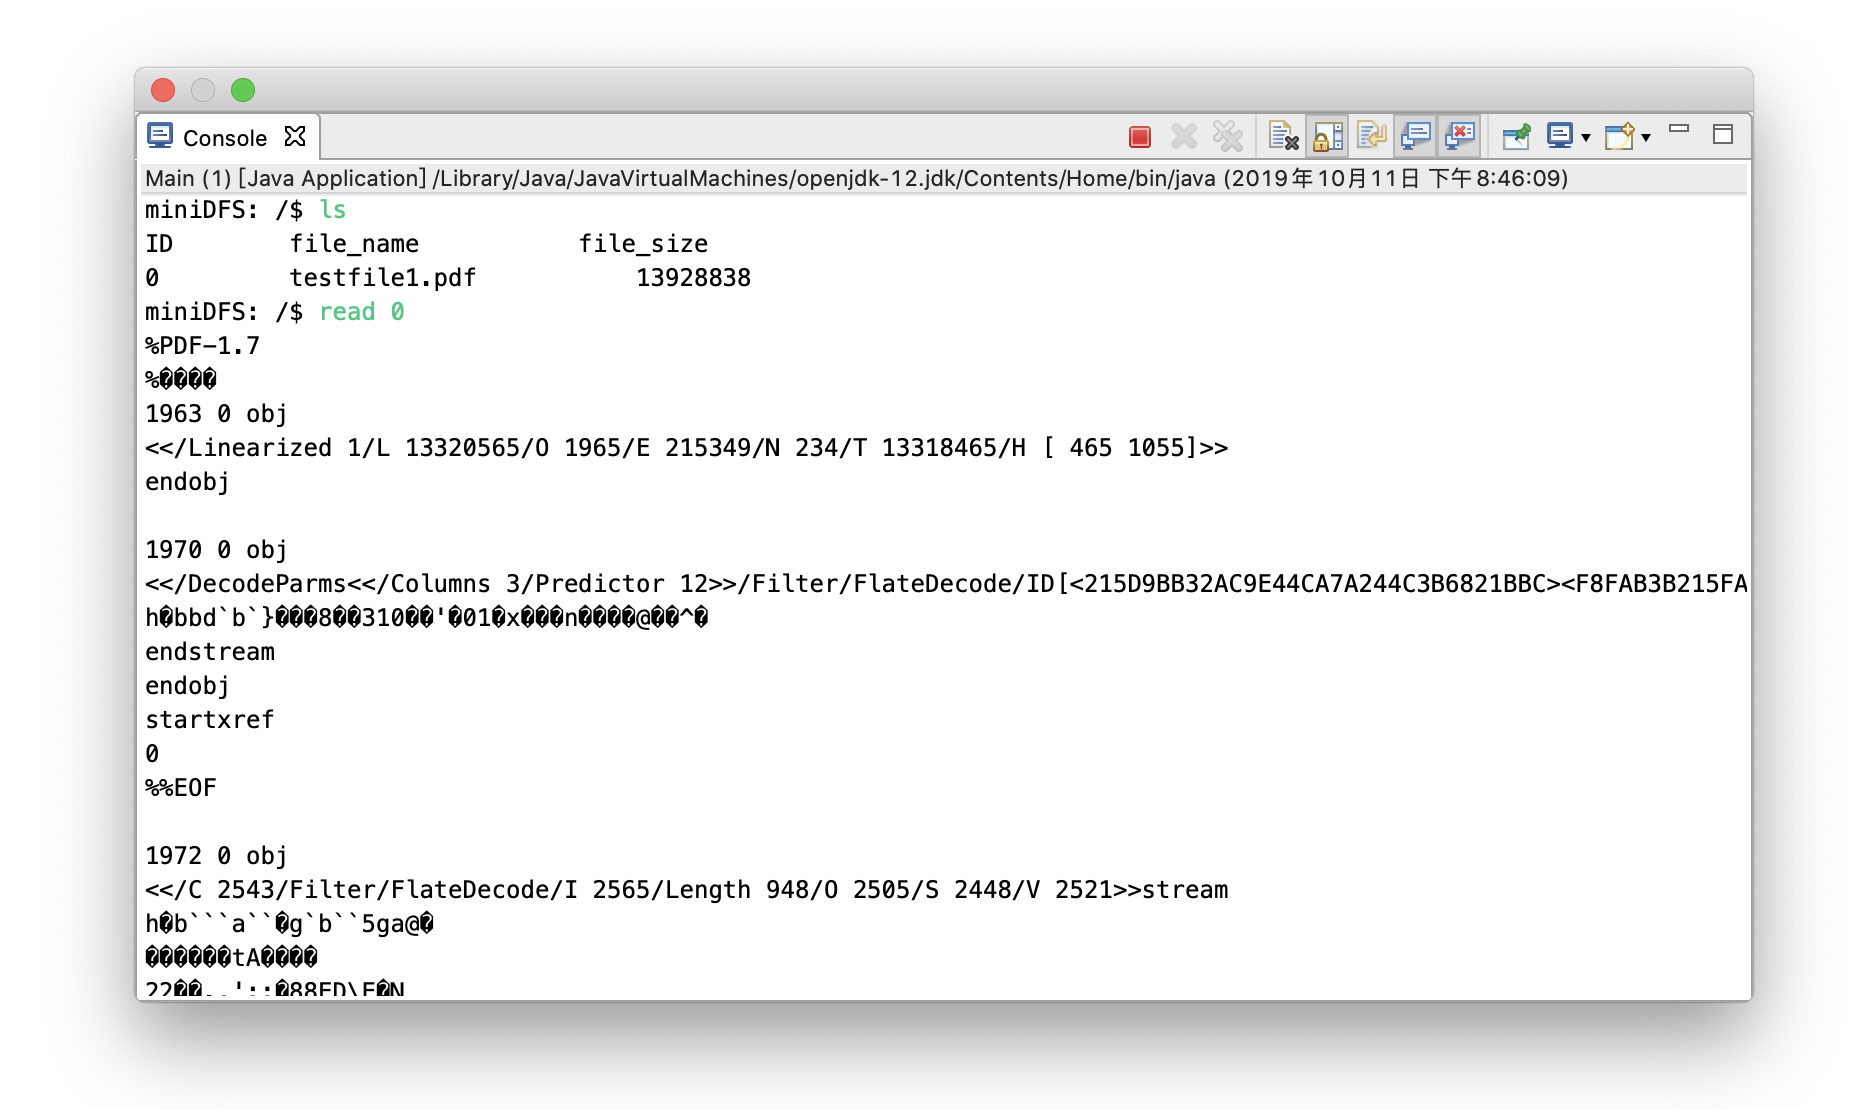
\includegraphics[width = 1\textwidth]{screenshot//read_01.png}}
\caption{Usage: read}
% \label{fig_process}
\end{figure}

Next, we download this file to local file system: directory \textit{./dfs} .
This could be any directory on the client side. We choose \textit{./dfs} just because
it is easier to demonstrate the changes on the disk.

\begin{figure}[H]
\centerline{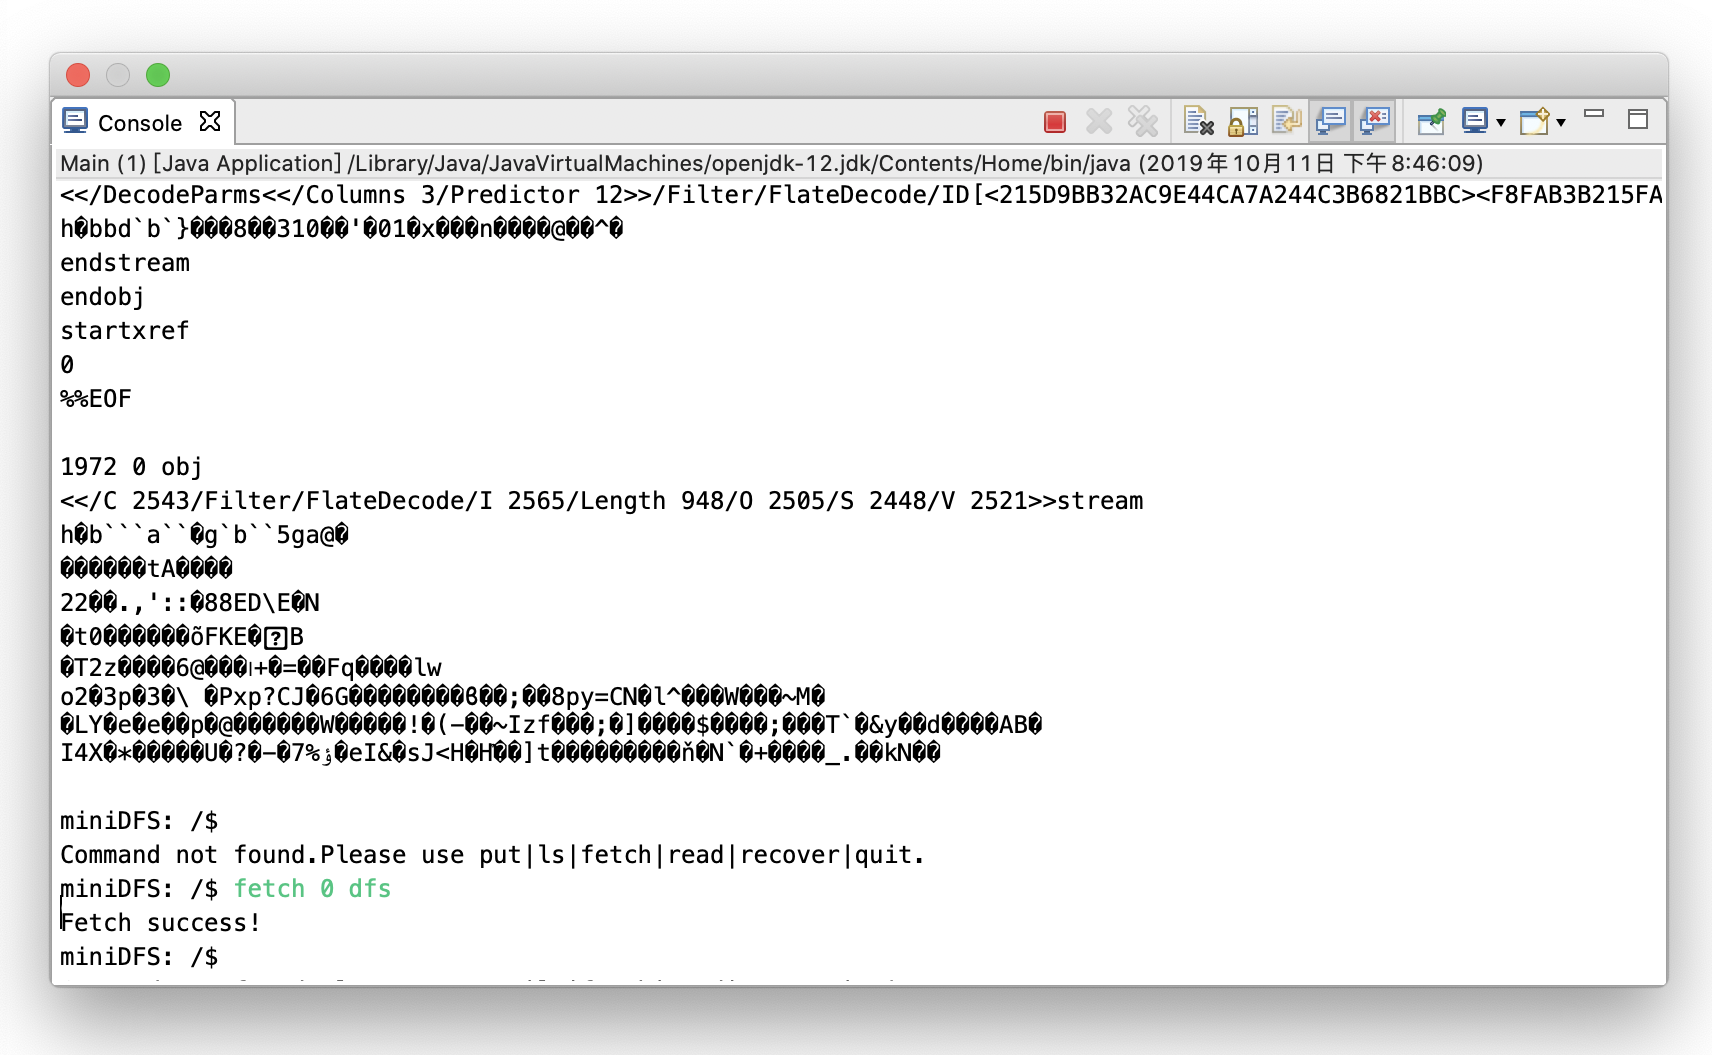
\includegraphics[width = 1\textwidth]{screenshot//fetch_01.png}}
\caption{Usage: fetch}
% \label{fig_process}
\end{figure}

Well, it appears in the file system. The file is succefully downloaded from the Mini-DFS.
As you could probably see from the picture, this is an e-book about body training.

\begin{figure}[H]
\centerline{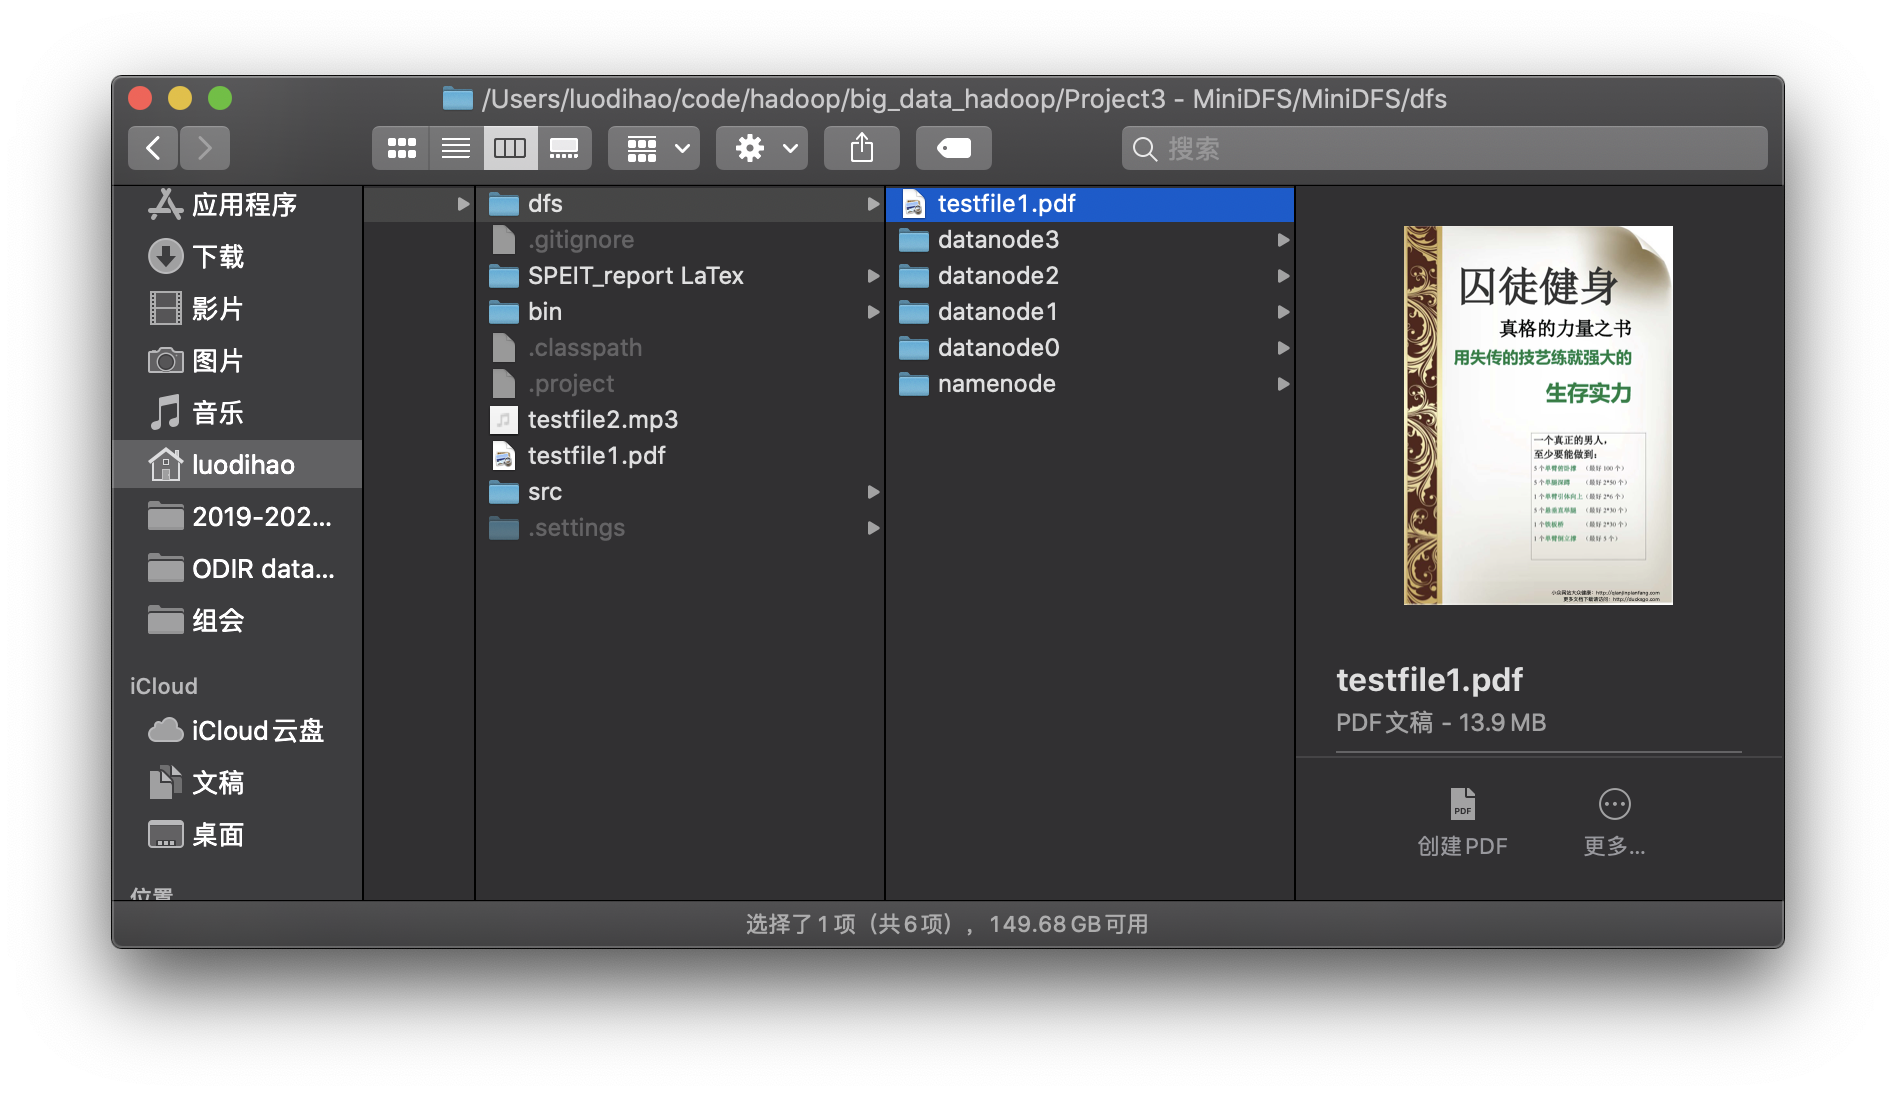
\includegraphics[width = 1\textwidth]{screenshot//fetch_02.png}}
\caption{Usage: fetch}
% \label{fig_process}
\end{figure}

Then, we delete \textit{datanode0} and try to recover it. Remember, there should be at least
one replica of the \textit{datanode0} in Mini-DFS.

\begin{figure}[H]
\centerline{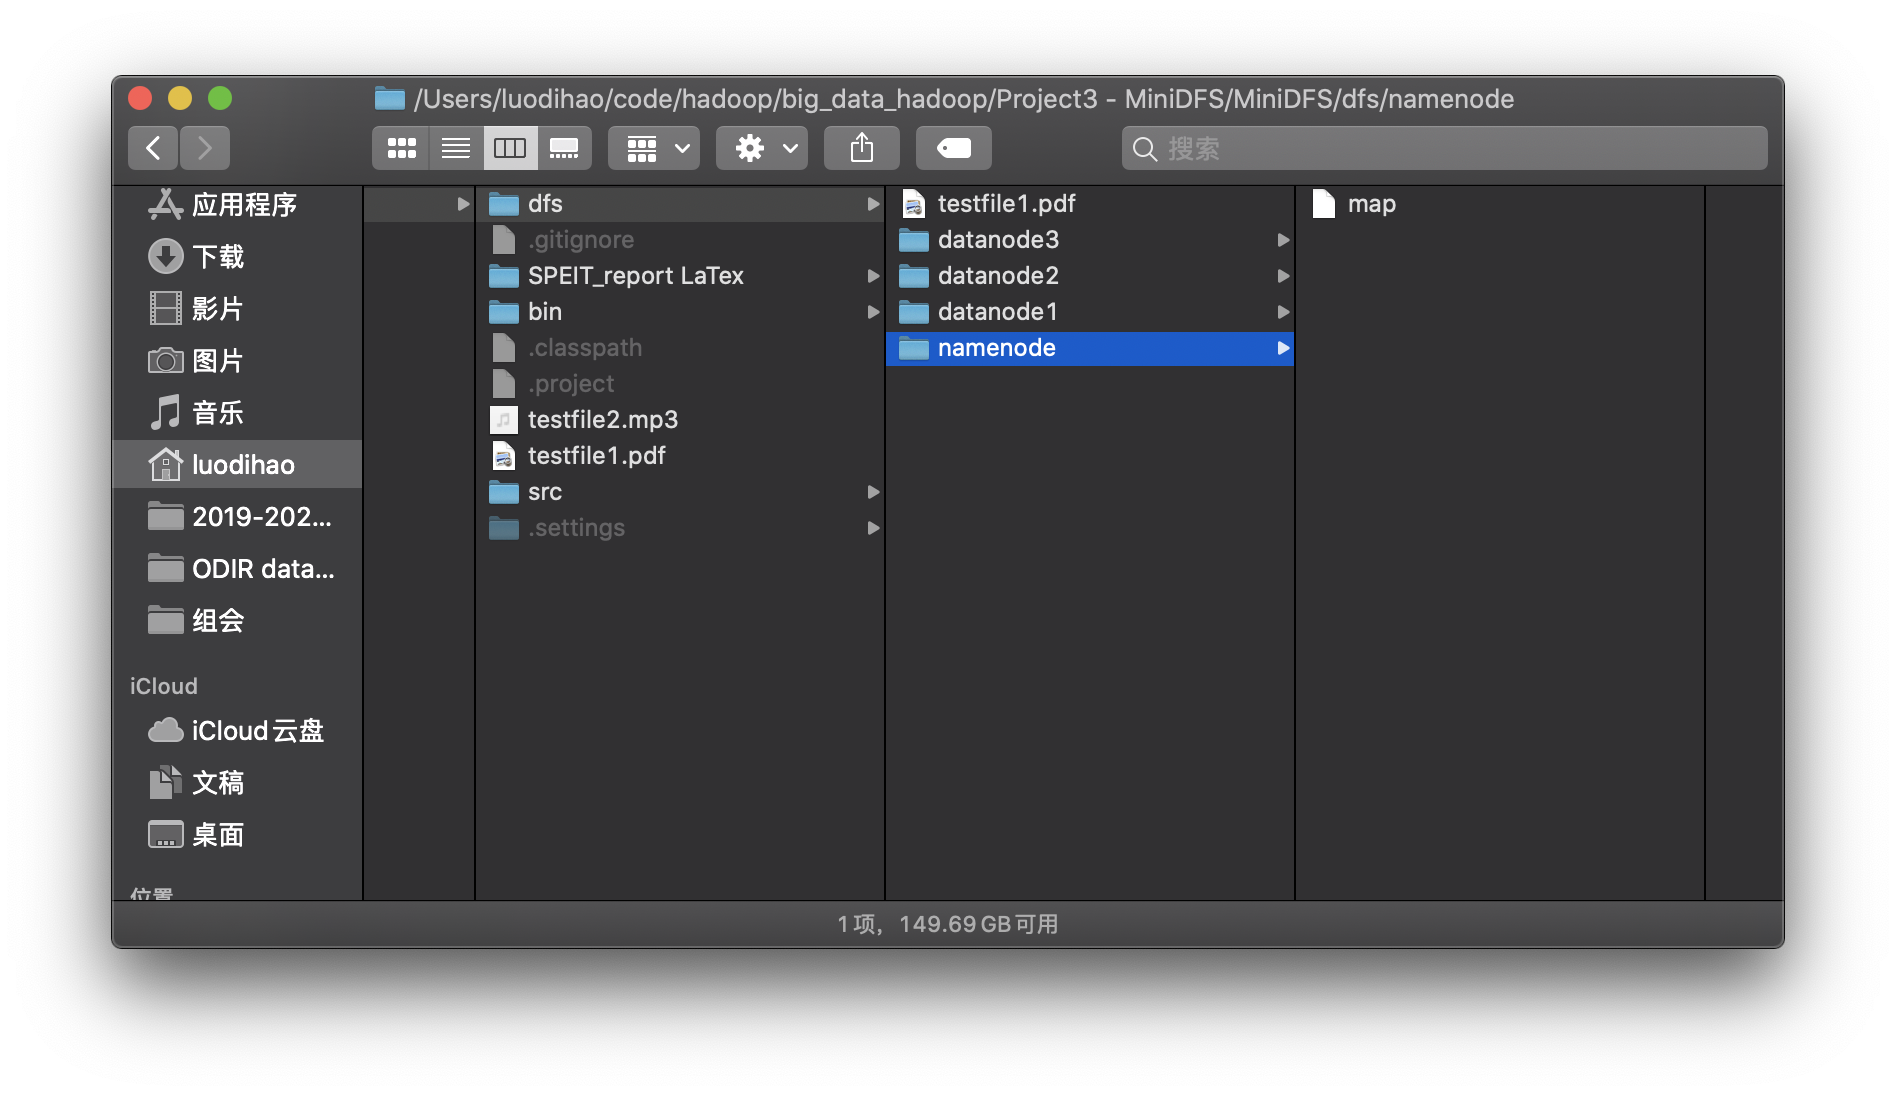
\includegraphics[width = 1\textwidth]{screenshot//recover_01.png}}
\caption{Usage: recover}
% \label{fig_process}
\end{figure}

Using \textit{recover 0}. The command will check the completency of the file 0.
Since Mini-DFS has the list of the server which should store the distributed data nodes,
it could safely check whether the corresponding data nodes still exist. If this is
not the case, it trys to find one replica to recover it.

\begin{figure}[H]
\centerline{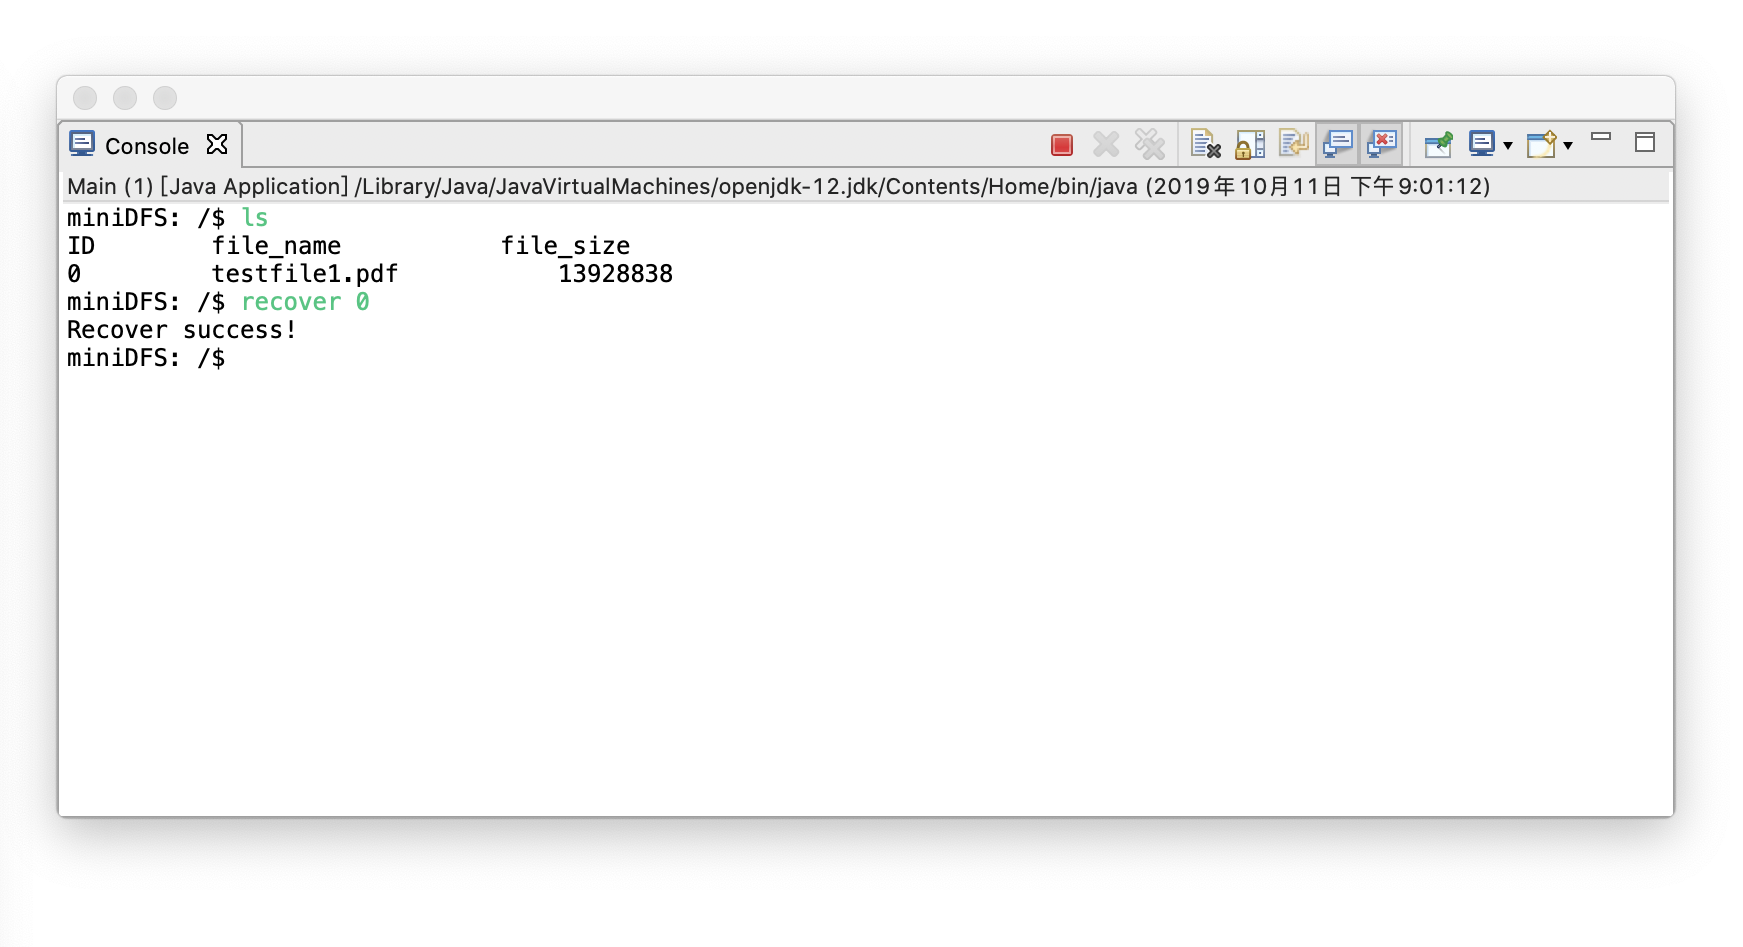
\includegraphics[width = 1\textwidth]{screenshot//recover_02.png}}
\caption{Usage: recover}
% \label{fig_process}
\end{figure}

It appears again in directory \textit{./dfs/} . The recovery will fail if there is no at least one replica, which makes sense.

\begin{figure}[H]
\centerline{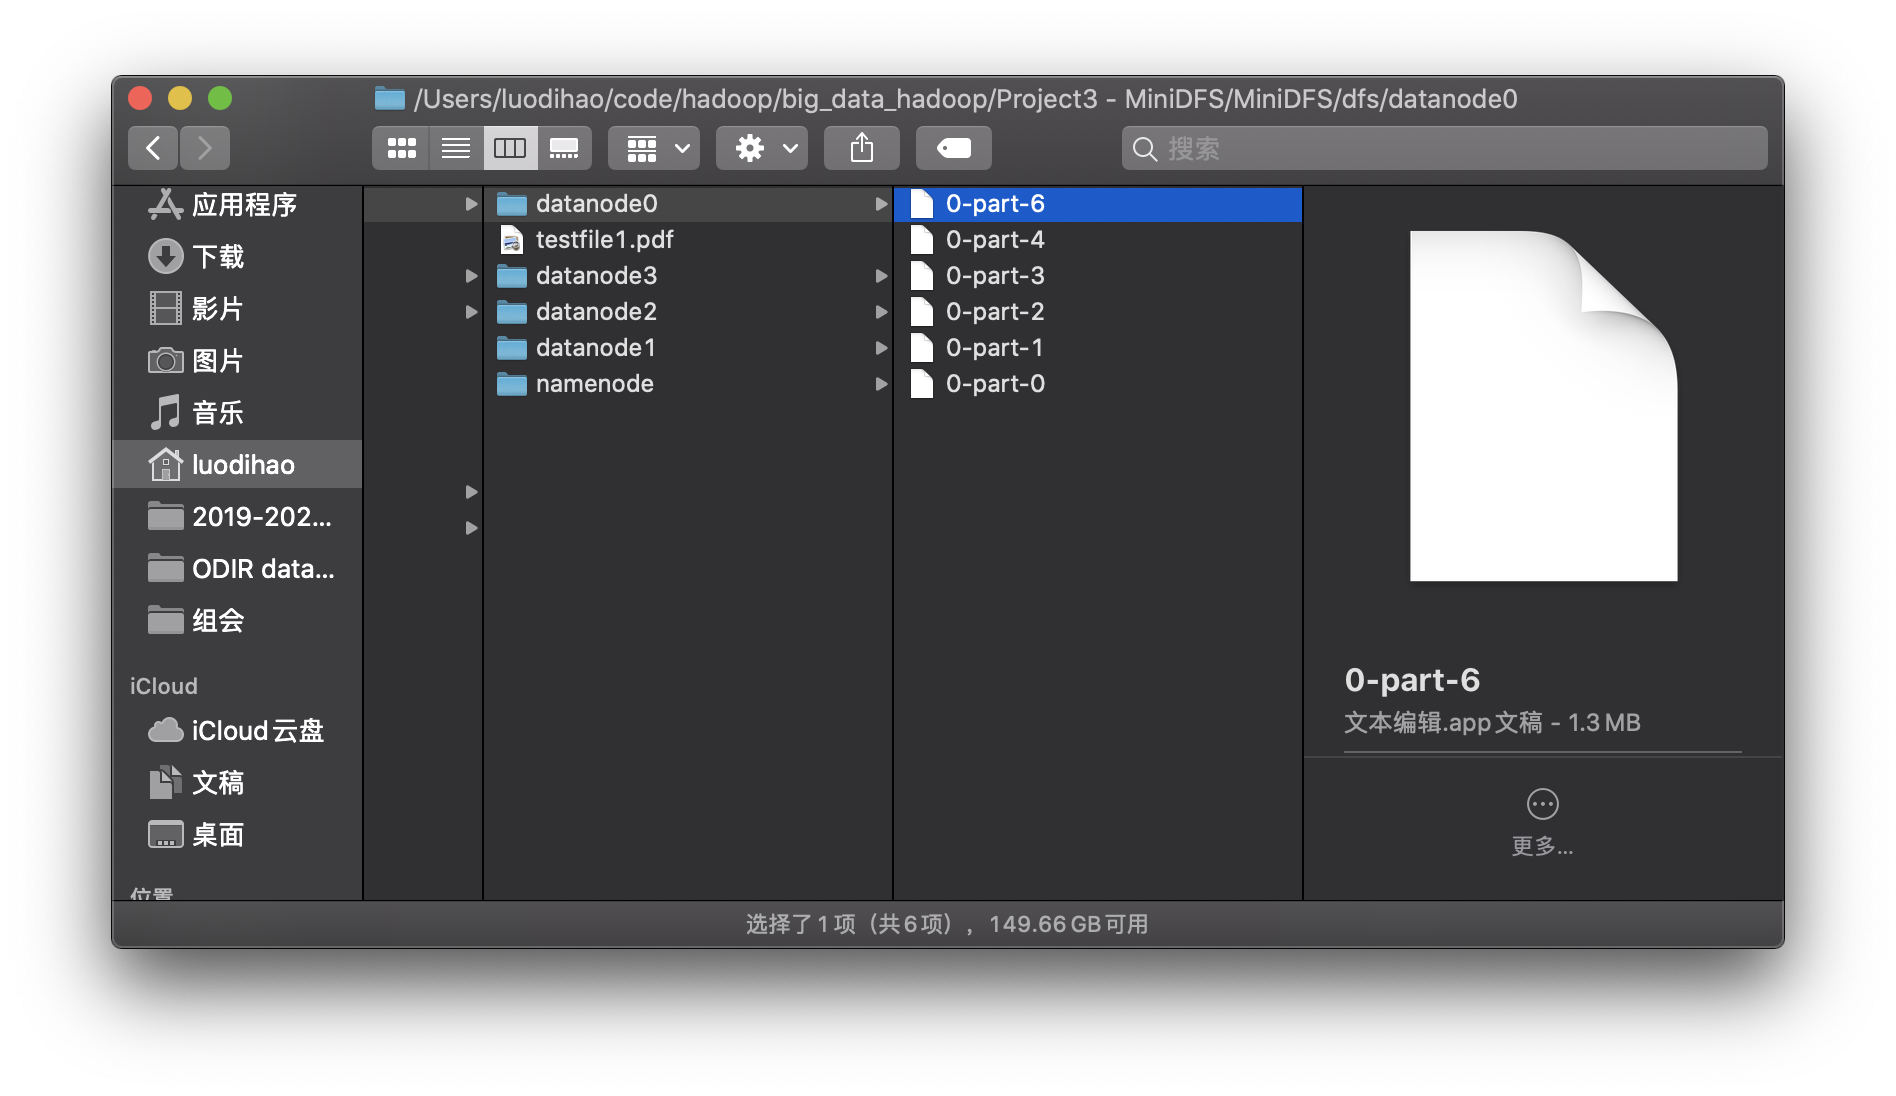
\includegraphics[width = 1\textwidth]{screenshot//recover_03.png}}
\caption{Usage: recover}
% \label{fig_process}
\end{figure}

Finally, we can safely exit Mini-DFS and this completes our examples of the experiment.

\begin{figure}[H]
\centerline{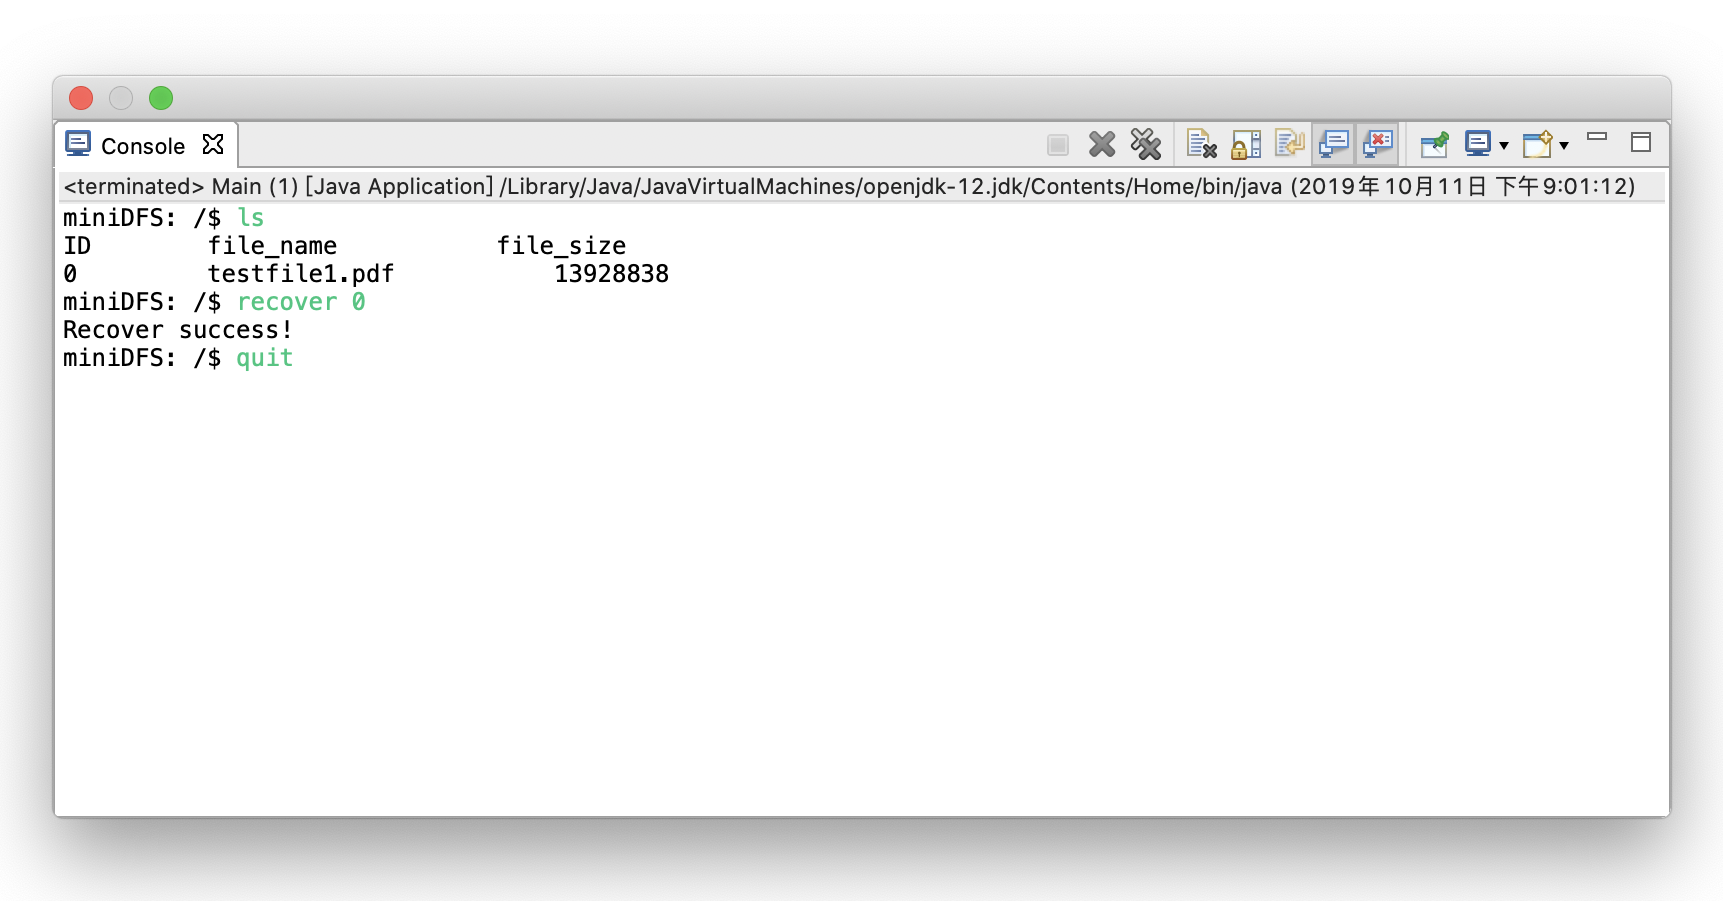
\includegraphics[width = 1\textwidth]{screenshot//quit_01.png}}
\caption{Usage: quit}
% \label{fig_process}
\end{figure}

% \begin{figure}[h]
% \centerline{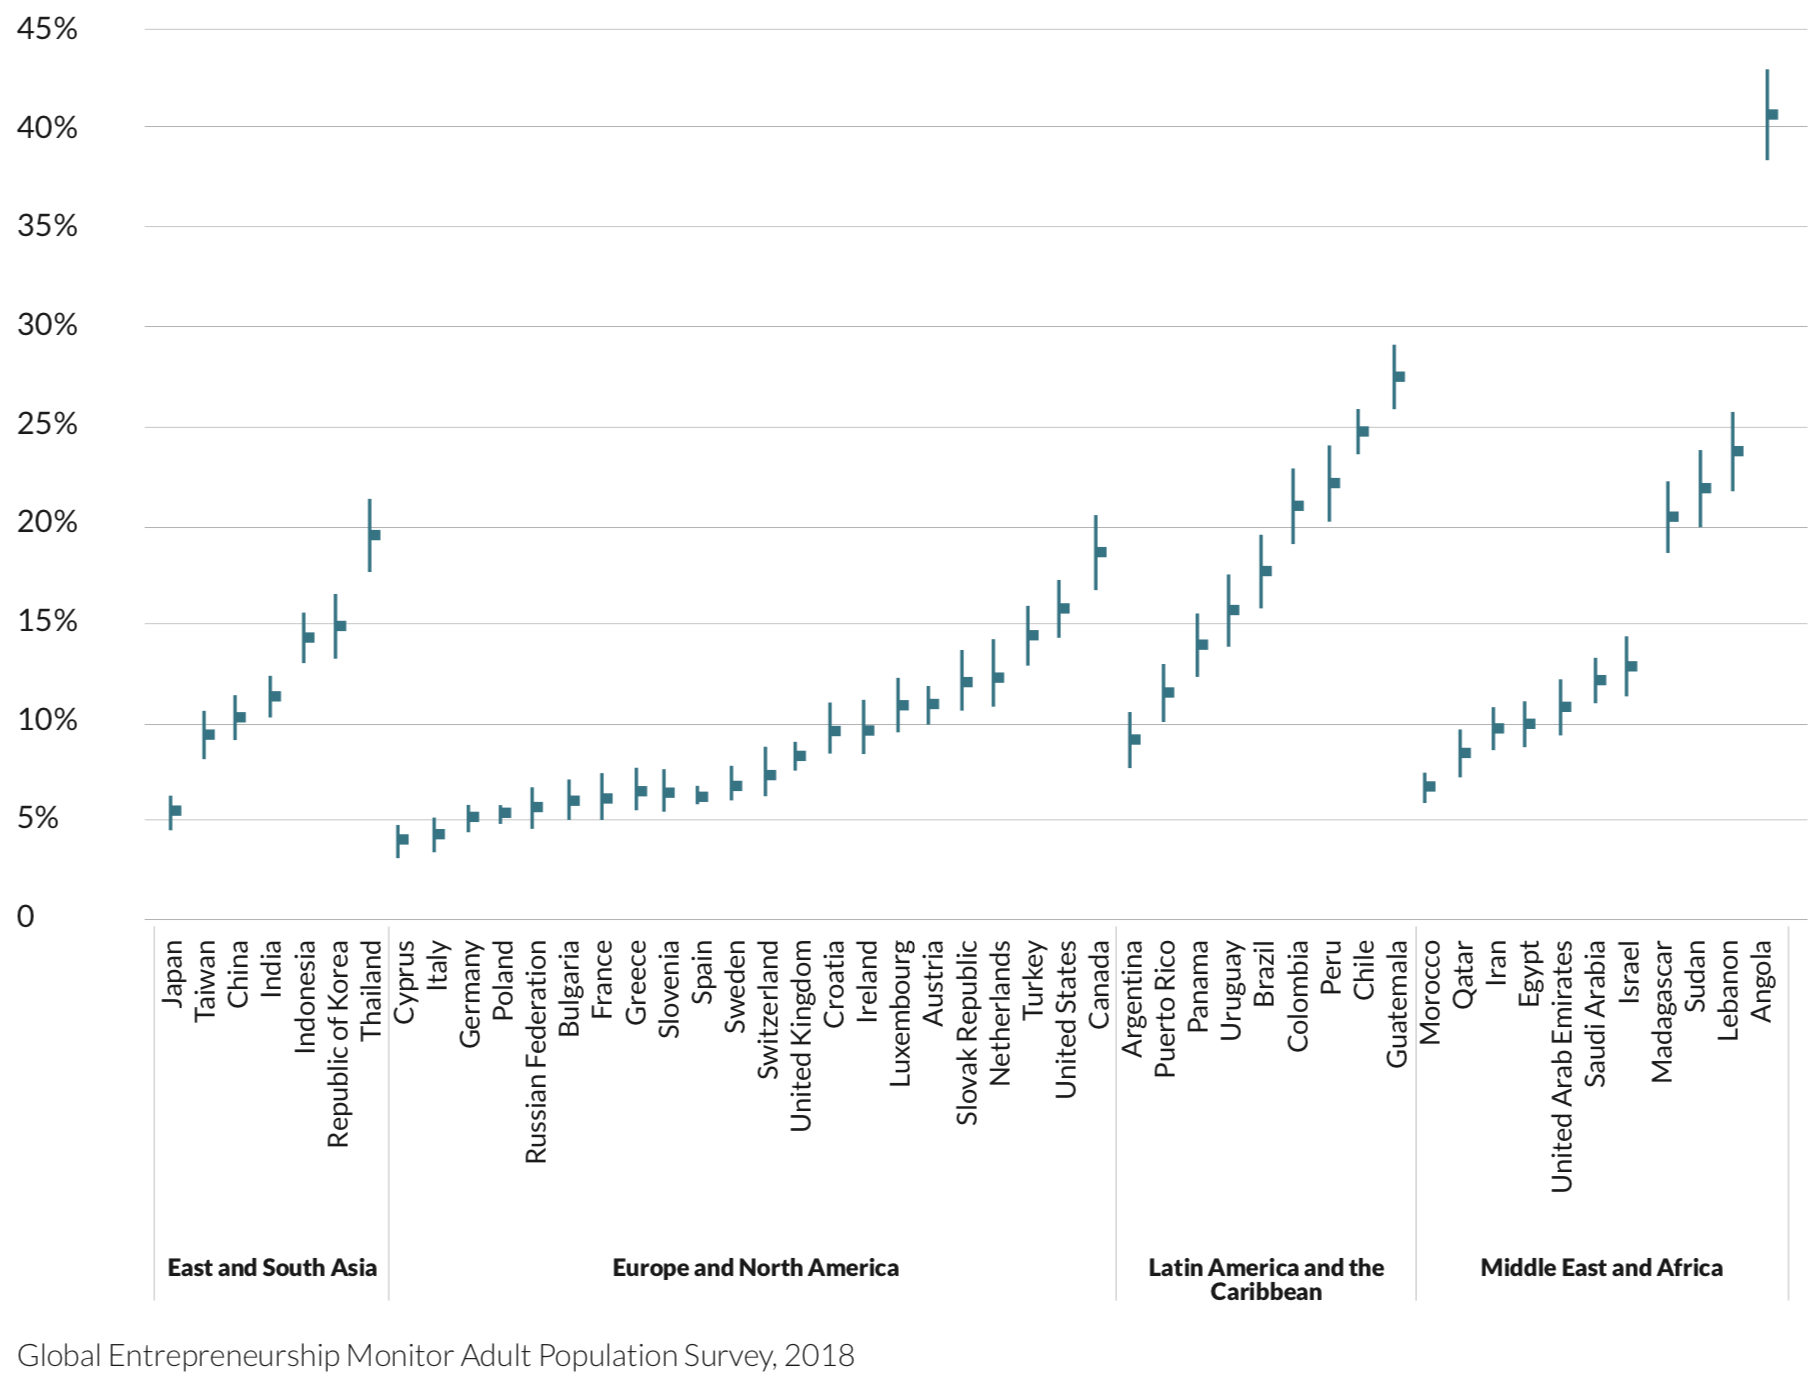
\includegraphics[width = 1\textwidth]{screenshot//2_2.png}}
% \caption{Total early-stage Entrepreneurial Activity (TEA) Rates among Adults (ages 18-64) in 487 Economies, in Four Geographic Regions}
% \label{fig_TEA_global}
% \end{figure}

% \section{Pod}
% \subsection{1 Pod with 1 Container}
%
% We can see after creating pod1 by pod1.yaml, we can execute any command by kubectl exec -it pod1 -- command.
%
% \begin{figure}[H]
% \centerline{\includegraphics[width = 0.7\textwidth]{screenshot//1.png}}
% \caption{1 Pod with 1 Container}
% % \label{fig_1pod1container}
% \end{figure}
%
% \subsection{1 Pod with 2 Containers}
%
% We can see after we change index.html in container ct-debian, we can also see the change in container ct-nginx.
%
% \begin{figure}[H]
% \centerline{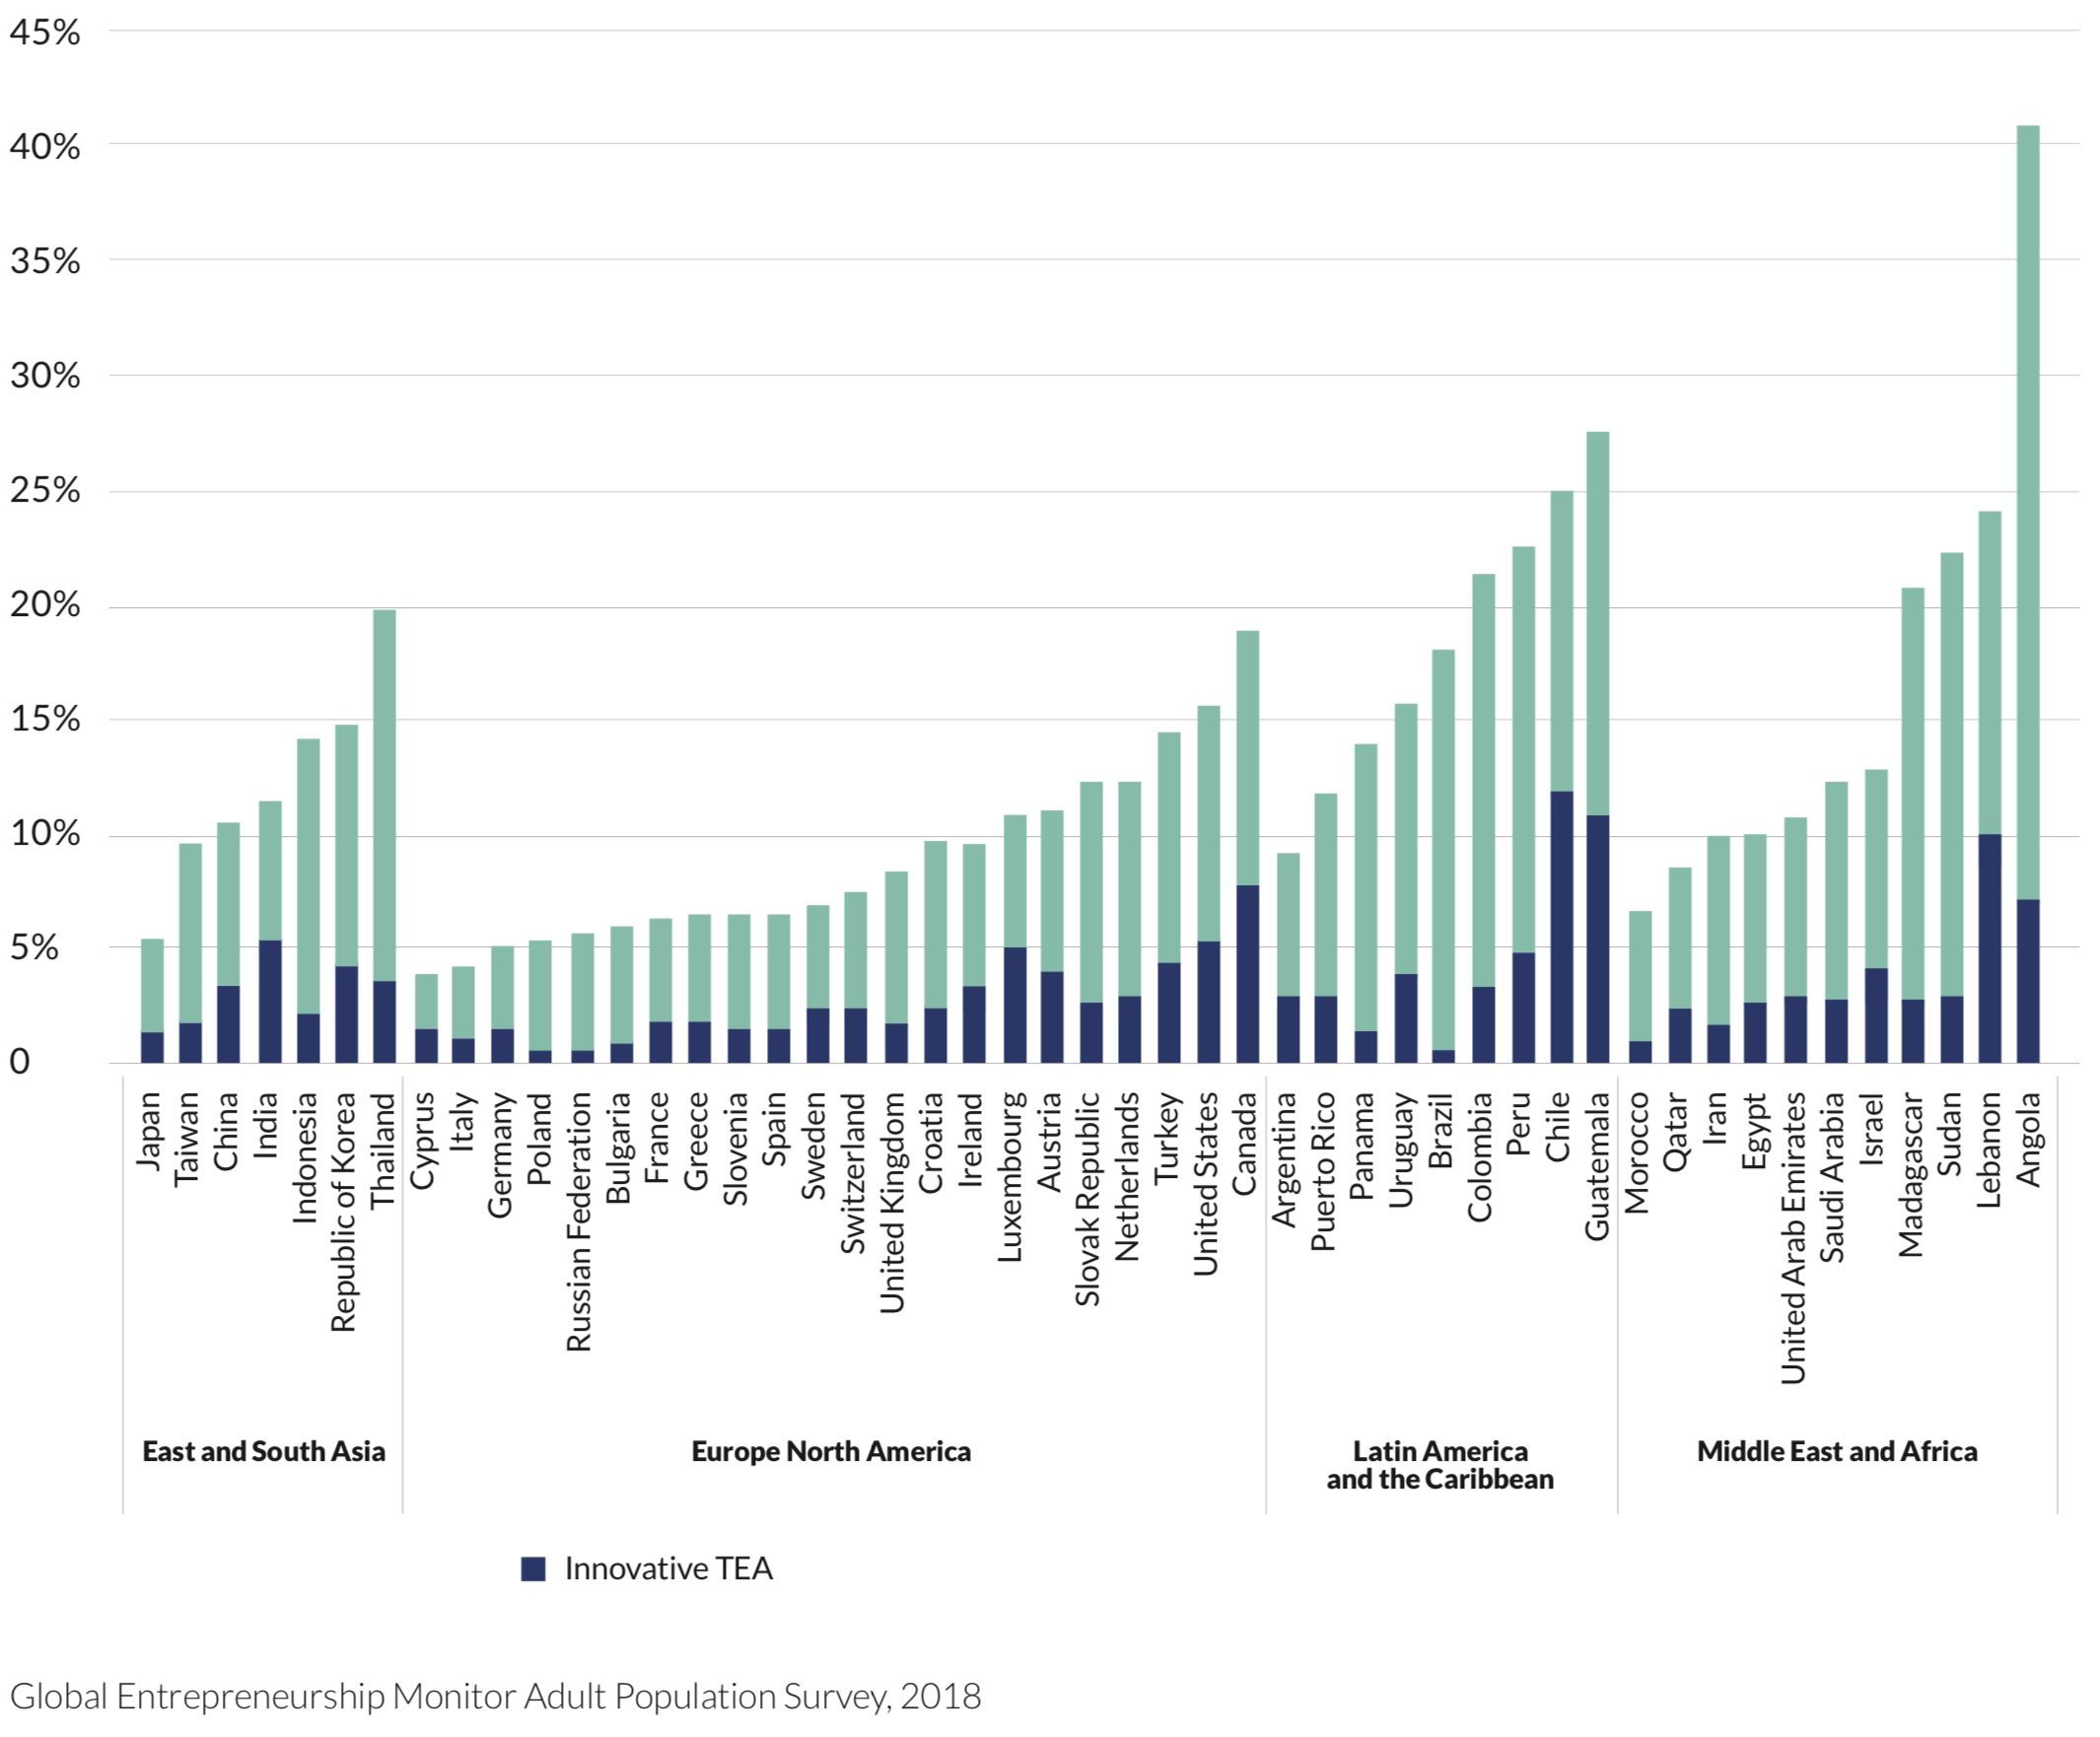
\includegraphics[width = 0.7\textwidth]{screenshot//2_1.png}}
% \caption{1 Pod with 2 Container}
% % \label{fig_1pod1container}
% \end{figure}






\end{document}
